\chapter{Arquitetura}
\paragraph{}

A arquitetura do projeto é representada na Figura \ref{fig:Arquitetura}. Este ilustra os caminhos de migração do \textbf{Oracle SQL} para o \textbf{MongoDB} e \textbf{Neo4j}, e destaca a fase de exploração para cada sistema de bases de dados.

\begin{itemize}
    \item \textbf{Oracle SQL}: A base de dados relacional de origem, contendo várias tabelas como pacientes, staff, episódios, entre outras, que representam os dados do hospital.
    \item \textbf{MongoDB}: Uma base de dados orientada a documentos onde os dados são armazenados em documentos flexíveis, semelhantes a JSON. Este sistema é utilizado para gerir a natureza semi-estruturada e hierárquica dos dados do hospital.
    \item \textbf{Neo4j}: Uma base de dados orientada a grafos, desenhada para gerir dados altamente conectados. É empregada para representar as relações complexas entre diferentes entidades dentro1 do sistema hospitalar.
\end{itemize}

Os principais objetivos deste projeto incluem a \textbf{Migração de Dados}, a \textbf{Exploração do Sistema} e a \textbf{Análise Crítica}. A migração de dados consiste em transferir informações de uma base de dados Oracle SQL existente, que armazena dados de um sistema de gestão hospitalar, para MongoDB e Neo4j. Este processo envolve compreender a estrutura dos dados, definir as transformações necessárias e implementar scripts para facilitar a transferência.

A exploração do sistema visa implementar um conjunto de consultas para demonstrar as capacidades operacionais dos novos sistemas não relacionais. Isto envolve investigar como os dados podem ser acedidos, manipulados e utilizados dentro do MongoDB e Neo4j, em comparação com a base de dados Oracle SQL original.

Por fim, a análise crítica foca-se em realizar uma comparação dos modelos de bases de dados relacionais e não relacionais, avaliando as vantagens, limitações e desempenho de cada sistema no tratamento dos dados do hospital.

\begin{figure}[H]
    \centering
    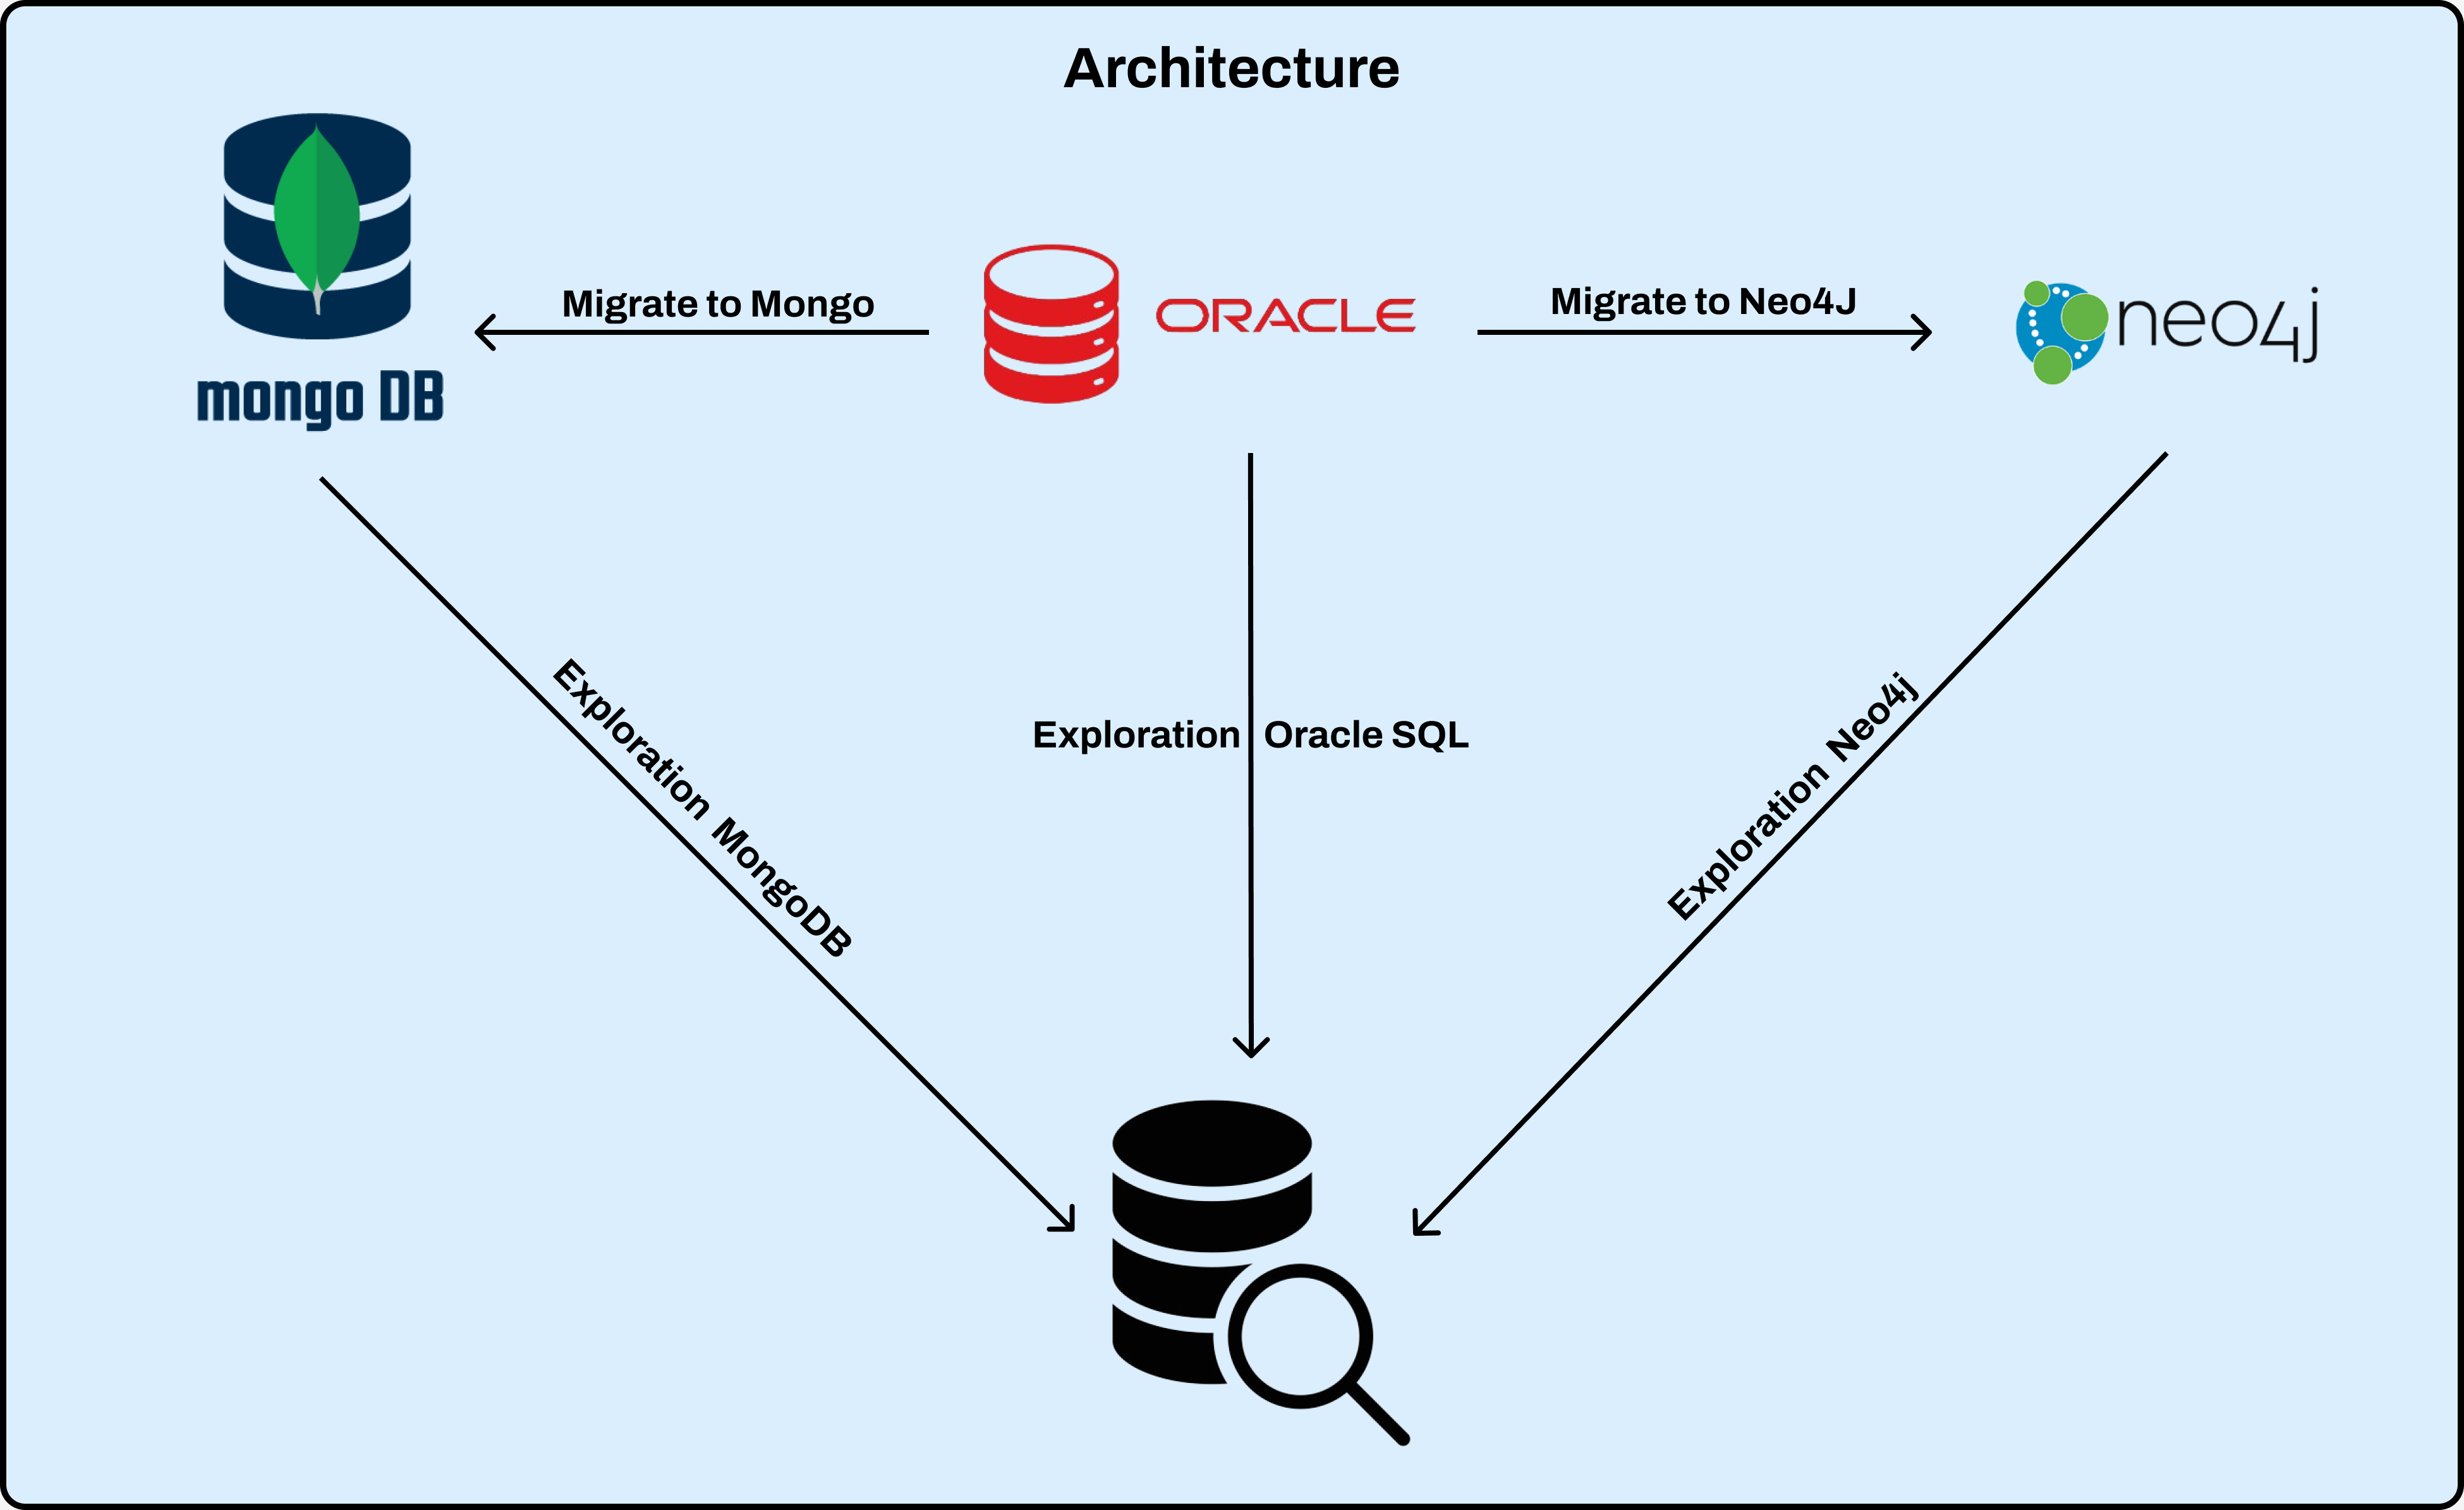
\includegraphics[width=0.8\linewidth]{Imagens/arquitetura.png}
    \caption{Arquitetura}
    \label{fig:Arquitetura}
\end{figure}

